\documentclass[conference]{IEEEtran}
\usepackage[T1]{fontenc}
\usepackage{times}
\usepackage{amsmath,amssymb}
\usepackage{graphicx}
\usepackage{booktabs}
\usepackage{tabularx}
\usepackage{cite}
\usepackage{url}
\usepackage[hidelinks]{hyperref}
\hypersetup{pdftitle={Neural Q-Learning for an Episodic Stochastic Shortest-Path Problem},
pdfauthor={Chinmay Prashanth, Arjun Singh Yadav, Mohammad Ibrahim}}
\graphicspath{{../results/}}
\newcolumntype{L}{>{\raggedright\arraybackslash}X}
\newcommand{\code}[1]{\texttt{#1}}
\newcommand{\repo}{\href{https://github.com/arjunsinghyadav2/eee598-neural-q-learning}{%
\nolinkurl{github.com/arjunsinghyadav2/eee598-neural-q-learning}}}

\begin{document}

\title{Neural Q-Learning for an Episodic\\Stochastic Shortest-Path Problem}

\author{\IEEEauthorblockN{Chinmay Prashanth, Arjun Singh Yadav, Mohammad Ibrahim}
\IEEEauthorblockA{Team 9\\
EEE598, Arizona State University\\
cprashan@asu.edu, asyadav6@asu.edu, Mibrahe5@asu.edu}}

\maketitle

\begin{abstract}
We replace the Q table of our Assignment~2 learner with a feedforward network trained only
from sampled transitions of the same eight-state episodic stochastic shortest-path problem.
The network (one-hot 8--32--32--7, ReLU, 1575 parameters) masks infeasible actions when acting
and in the bootstrap, and learns with experience replay, a hard-copied target network and Adam
on a mean-squared temporal-difference loss. On five seeds of 5000 episodes, every seed learned
the optimal policy (exact expected cost 8.44), and 1000-episode greedy evaluations gave mean
costs of 8.414--8.463 with every episode reaching $h$. Tabular Q-learning gave the same policy
in under 1/70 of the training time, and a sweep on ten held-out seeds shows that the network matches
the table's stability only with replay. With one-hot inputs there is nothing to generalize
across, so the network brings no benefit at this scale.
\end{abstract}

\section{Problem and Environment Reuse}
The task is the episodic, undiscounted ($\gamma=1$) shortest-path problem of Assignment~2
\cite{a2}: states $a$--$h$, start $a$, terminal $h$ with a terminal bootstrap of 0. At $a$,
$b$ and $c$ the agent names an intended successor ($\mathit{Ab}$/$\mathit{Ac}$,
$\mathit{Ad}$/$\mathit{Ae}$, $\mathit{Ae}$/$\mathit{Af}$), reached with probability 0.8,
while the other branch occurs with probability 0.2; $d$, $e$, $f$ have the single action
$\mathit{Ag}$ and $g$ has $\mathit{Ah}$. A transition costs the edge of the branch actually
taken ($\mathit{ab}$~2, $\mathit{ac}$~2, $\mathit{bd}$~3, $\mathit{be}$~2, $\mathit{ce}$~5,
$\mathit{cf}$~4, $\mathit{dg}$~3, $\mathit{eg}$~3, $\mathit{fg}$~2, $\mathit{gh}$~1); cost
is minimized. Each episode has four steps and costs 8, 9 or 11.

\begin{table*}[t]
\caption{Hyperparameters of the Neural Learner and Their Justification}
\label{tab:hyper}
\centering\footnotesize
\setlength{\tabcolsep}{4pt}
\begin{tabularx}{\textwidth}{@{}l l L@{}}
\toprule
Item & Value & Justification\\
\midrule
Network & 8--32--32--7, ReLU, linear out & assignment default, 1575 parameters; $8\times8$ (207), 32 (519), $128\times128$ (18{,}567) also learn $\pi^*$\\
Loss & MSE, Eq.~(2) & $Q$ is the target's mean; Huber ($\delta=1$) pulls $Q(c,\cdot)$ 0.15 toward the likelier branch (Q RMSE 0.113)\\
Optimizer & Adam, lr $10^{-3}$ & assignment default; lr $10^{-4}$ settles $6\times$ later (episode 686), lr $10^{-2}$ leaves late switches\\
Batch size & 32 & batch 8 raises the Q RMSE $1.7\times$; 128 lowers it 16\% for $4\times$ the samples per step\\
Replay capacity & 10{,}000 transitions & $\approx$2500 episodes of history keep rare pairs; 500 or no replay: 8.5--8.7 late switches\\
Warm-up & 200 transitions & not swept; 50 near-random episodes give an expected 12.5 visits to each rarest pair\\
Target copy & every $M=100$ learning steps & 198 copies per run; $M=1$ raises the Q RMSE $2.2\times$, $M=2000$ settles $3\times$ later\\
Exploration & $\varepsilon$: $1\to0.05$ over episodes 1--4000 & assignment default; a constant $\varepsilon=0.02$ leaves 2.3 late switches\\
Length & 5000 episodes per seed & assignment default; every seed settles by episode 130 (1000 episodes also suffice)\\
Discount & $\gamma=1$, terminal bootstrap 0 & episodic; every episode ends after 4 steps\\
Other & PyTorch defaults & Adam $\beta=(0.9,0.999)$, stabilizer $10^{-8}$; weights and biases drawn from $U(\pm1/\sqrt{\text{fan-in}})$\\
Seeds & 0--4, all state rebuilt per seed & reported seeds are never used for tuning (held-out seeds 100--109)\\
Evaluation & 1000 episodes, $\varepsilon=0$ & noise from \code{SeedSequence([598003,seed])}, apart from all training streams\\
\bottomrule
\end{tabularx}
\\[2pt]
\parbox{\textwidth}{\footnotesize Sweep values: means over held-out seeds 100--109 (settling
episodes: medians); defaults: Q RMSE 0.082, no late switches, settling at episode 112. Q RMSE:
root-mean-square error of the 10 $Q$ values against $Q^*$. Late switches: changes of the greedy
$(a,b,c)$ actions in the last 1000 episodes. Settling: first episode from which the policy stays
$\pi^*$.}
\end{table*}

\emph{Reuse and checks.} States, action sets, transition table and sampler are copied
verbatim from our Assignment~2 code. The learner sees only an environment object whose
\code{step(a)} returns a sampled $(s',c,\text{terminal})$, raising an error on an infeasible
action or after $h$, and whose \code{feasible\_actions(s)} lists the legal actions. Before
every experiment, 149 self-checks run. For the environment they confirm the probabilities and
edge costs, branch frequencies within 0.0132 of their probabilities over 8000 episodes,
four-step episodes costing 8, 9 or 11, errors on illegal calls, and that the reused tabular
learner reproduces the Assignment~2 Q tables and costs bit for bit on seeds 0--4. Policy
iteration \cite{si6} gives the reference $V^*(a)=8.44$, $\pi^*$: $a\to\mathit{Ab}$,
$b\to\mathit{Ae}$, $c\to\mathit{Af}$ and $Q^*(a,\cdot)=(8.44,9.16)$, $Q^*(b,\cdot)=(6.8,6.2)$,
$Q^*(c,\cdot)=(8.6,7.4)$, used only after training: model-based functions raise errors while a
learner trains, and training with the transition table hidden from all but the sampler gives
identical weights.

\section{Neural Q-Function}
\emph{Architecture.} The input is the one-hot encoding of the state (8 units, order
$a$--$h$). Two fully connected hidden layers of 32 ReLU units feed 7 linear outputs, one per
action label in the order $\mathit{Ab}, \mathit{Ac}, \mathit{Ad}, \mathit{Ae}, \mathit{Af},
\mathit{Ag}, \mathit{Ah}$. Output $j$ estimates $Q(s,a_j)$, the expected total cost to reach
$h$ after taking $a_j$ in $s$, so smaller is better; the outputs are linear so that no
activation bounds the cost-to-go. The network has
$(8\cdot32+32)+(32\cdot32+32)+(32\cdot7+7)=288+1056+231=1575$ trainable parameters, against
10 entries in the table.

\emph{Masking.} A Boolean $8\times7$ mask $F$ marks the 10 feasible state--action pairs (from
\code{feasible\_actions}); the row of $h$ is empty. The greedy action is
$\arg\min_{a:F(s,a)}Q(s,a)$ with exact ties broken uniformly at random, and random
$\varepsilon$ actions are drawn uniformly from the feasible actions. In the bootstrap,
infeasible outputs are set to $+\infty$ before the minimum, and terminal transitions receive a
bootstrap of exactly 0 through a select (\code{torch.where}), because multiplying the
$+\infty$ minimum of the all-masked $h$ row by 0 would give NaN. Only the output of the action
taken enters the loss, so infeasible outputs are never trained and never used.

\section{Learning Algorithm}
Each environment step stores $(s,a,c,s',\text{terminal})$ in a 10{,}000-transition ring
buffer \cite{lin92}. Once 200 transitions are stored, every environment step performs one
learning step on $B=32$ transitions drawn uniformly with replacement:
\begin{align}
y_i &= \begin{cases} c_i & \text{if } s'_i=h,\\
c_i+\gamma\min_{a':F(s'_i,a')}Q_{\theta^-}(s'_i,a') & \text{otherwise,}\end{cases}\\
L(\theta) &= \frac{1}{B}\sum_{i=1}^{B}\bigl(y_i-Q_\theta(s_i,a_i)\bigr)^2,
\end{align}
where $\theta^-$ is a separate target network. Adam \cite{adam} with learning rate (lr)
$10^{-3}$ updates $\theta$, and $\theta^-\leftarrow\theta$ is a hard copy every $M=100$
learning steps \cite{dqn}. Actions at $a$, $b$, $c$ are $\varepsilon$-greedy on the online
network, with $\varepsilon_k=1-0.95(k-1)/3999$ in episode $k\le4000$ and 0.05 afterwards. A
seed's 5000 episodes give 20{,}000 transitions, 19{,}801 learning steps and 198 target copies.
For every seed 0--4 the network, target, optimizer, buffer and $\varepsilon$ schedule are
rebuilt; \code{torch}, \code{numpy} and \code{random} are seeded with the seed, and
\code{SeedSequence(seed)} spawns independent streams for environment noise, exploration and
replay sampling; training runs on one CPU thread. Table~\ref{tab:hyper} justifies each value,
mostly with the one-factor sweep of Section~\ref{sec:compare}, which used only held-out seeds.

\section{Results}
\begin{figure}[t]
\centering
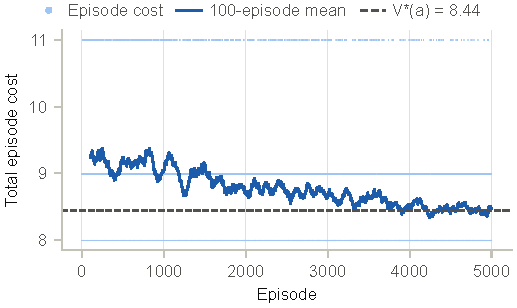
\includegraphics[width=0.94\columnwidth]{fig_seed4_cost.pdf}
\caption{Seed 4: total cost of each training episode (dots; only 8, 9 and 11 occur) and its
100-episode rolling mean. Dashed: optimal expected cost $V^*(a)=8.44$; with
$\varepsilon=0.05$ the expected training cost of $\pi^*$ is 8.48.}
\label{fig:cost}
\end{figure}

\begin{figure}[t]
\centering
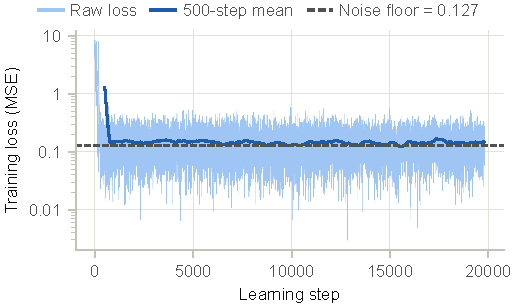
\includegraphics[width=0.94\columnwidth]{fig_seed4_loss.pdf}
\caption{Seed 4: minibatch mean-squared-error (MSE) loss of every learning step (log scale) and
its 500-step rolling mean. Dashed: expected loss at $Q=Q^*$ for the final buffer's mix of pairs,
$\sum_{s,a}\mathrm{freq}(s,a)\,\mathrm{Var}[c+V^*(s')\,|\,s,a]$; sampled targets keep the loss
from reaching zero.}
\label{fig:loss}
\end{figure}

\begin{table}[t]
\caption{Neural Greedy Policy and 1000-Episode Evaluation per Seed}
\label{tab:eval}
\centering\footnotesize
\setlength{\tabcolsep}{2.5pt}
\begin{tabular}{@{}c c c c c c c c@{}}
\toprule
Seed & $\pi(a,b,c)$ & Nom.\ path & Mean & SD & Min--max & \% $h$ & Q RMSE\\
\midrule
0 & $\mathit{Ab},\mathit{Ae},\mathit{Af}$ & $\mathit{abegh}$, 8 & 8.429 & 0.697 & 8--11 & 100 & 0.106\\
1 & $\mathit{Ab},\mathit{Ae},\mathit{Af}$ & $\mathit{abegh}$, 8 & 8.463 & 0.721 & 8--11 & 100 & 0.088\\
2 & $\mathit{Ab},\mathit{Ae},\mathit{Af}$ & $\mathit{abegh}$, 8 & 8.414 & 0.632 & 8--11 & 100 & 0.084\\
3 & $\mathit{Ab},\mathit{Ae},\mathit{Af}$ & $\mathit{abegh}$, 8 & 8.441 & 0.672 & 8--11 & 100 & 0.094\\
4 & $\mathit{Ab},\mathit{Ae},\mathit{Af}$ & $\mathit{abegh}$, 8 & 8.428 & 0.679 & 8--11 & 100 & 0.081\\
\midrule
\multicolumn{3}{@{}l}{Mean $\pm$ SD over seeds} & 8.435 & 0.680 & & 100 & 0.091\\
\multicolumn{3}{@{}l}{} & $\pm$0.018 & $\pm$0.033 & & & $\pm$0.010\\
\bottomrule
\end{tabular}
\\[2pt]
\parbox{\columnwidth}{\footnotesize Every seed: $\mathit{Ag}$ at $d,e,f$ and $\mathit{Ah}$ at
$g$; exact $V^\pi(a)=8.44$ (gap 0); 95\% half width of each mean $\approx0.04$; SD: sample
standard deviation.}
\end{table}

\begin{table*}[t]
\caption{Neural Versus Tabular Q-Learning on Seeds 0--4 (Times per Seed). Tabular
$x$\,/\,$y$: Assignment~2 (A2)\,/\,Matched Schedule}
\label{tab:compare}
\centering\footnotesize
\begin{tabularx}{\textwidth}{@{}l >{\raggedright\arraybackslash\hsize=1.12\hsize}X
>{\raggedright\arraybackslash\hsize=0.88\hsize}X@{}}
\toprule
Aspect & Neural Q-function (this work) & Tabular Q-learning\\
\midrule
Representation & 1575 shared weights; one-hot inputs leave nothing to generalize over & 10 independent entries, one per feasible pair\\
Model access & sampled $(s,a,c,s',\text{terminal})$ only; model functions raise in training & same\\
Sampling & replayed $\approx$32 times on average; Q RMSE $<0.3$ by episode 111--137 & used once; Q RMSE $<0.3$ by episode 147--185\\
Exploration & $\varepsilon$-greedy at $a,b,c$: $1\to0.05$ over episodes 1--4000 & same rule; A2 decays over the first 2000 episodes\\
Stability & no late switches on seeds 0--4 or 100--109; 8.7 without replay & 2\,/\,6 late switches on seed 3; none on seeds 100--109\\
Reproducibility & seeded initialization, 3 streams, 1 thread; hashes repeat on one build & one generator; equals Assignment~2 bit for bit\\
Sensitivity & lr, $\varepsilon$, layers, batch, replay, $M$, loss, length; $\pi^*$ in every variant & $\alpha$, $\varepsilon$, length; $\alpha\ge0.5$ loses $\pi^*$ on 1--2 of 10 seeds\\
Policy and cost & $\pi^*$ on 5/5; mean $8.435\pm0.018$; Q RMSE $0.091\pm0.010$; 12.3~s &$\pi^*$ on 5/5; same eval.; Q RMSE 0.084/0.097; 0.17/0.16~s\\
\bottomrule
\end{tabularx}
\end{table*}

In Fig.~\ref{fig:cost} the 100-episode mean starts at 9.25, the expected cost of uniform
random actions, and falls toward 8.48, the expected cost of $\pi^*$ under 5\% exploration, as
$\varepsilon$ decays; the greedy policy is $\pi^*$ from episode 107 on. In Fig.~\ref{fig:loss}
the loss falls from about 7 to 0.15 within 750 learning steps and then hovers just above 0.127,
the expected squared error of sampled targets at $Q=Q^*$ for the final buffer. The plateau is
mostly target noise, not a failure to converge: over the last 1000 steps the mean loss is
0.127--0.146 across seeds, against expected values of 0.126--0.129.

Table~\ref{tab:eval} reports each seed's greedy policy and evaluation. Every seed learned
$\pi^*$: $a\to\mathit{Ab}$, $b\to\mathit{Ae}$, $c\to\mathit{Af}$, with the forced
$\mathit{Ag}$ at $d$, $e$, $f$ and $\mathit{Ah}$ at $g$. The nominal path, in which every
intended transition succeeds, is $a\to b\to e\to g\to h$ with cost 8, and the exact expected
cost is $V^\pi(a)=8.44=V^*(a)$. Each policy ran 1000 stochastic episodes with exploration off on
an environment stream separate from training. Every seed's 95\% interval contains 8.44, and the
standard deviations scatter around the exact 0.697 (costs 8, 9, 11 with probabilities 0.64,
0.32, 0.04). The three learners of Section~\ref{sec:compare} share each seed's evaluation
stream (common random numbers); as all learned $\pi^*$ on every seed, their evaluation columns are identical, and the spread
of the means across seeds is evaluation noise, not training variability.

\section{Neural Versus Tabular Q-Learning}
\label{sec:compare}
Table~\ref{tab:compare} compares the network with the tabular learner of Assignment~2 (step
size $\alpha=0.1$, $\varepsilon$ decayed over the first 2000 episodes) and with a matched
tabular baseline that uses the network's $\varepsilon$ in every episode; Fig.~\ref{fig:rmse}
follows their Q error.

\begin{figure}[t]
\centering
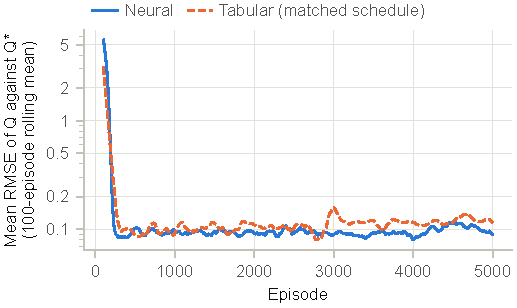
\includegraphics[width=0.94\columnwidth]{fig_q_rmse.pdf}
\caption{Seeds 0--4: RMSE of the 10 learned $Q$ values against $Q^*$, averaged over seeds, for
the network (solid) and the matched tabular learner (dashed); 100-episode rolling mean on a
log axis, so the curves start at episode 100. The network starts higher because it waits for
its 200-transition warm-up.}
\label{fig:rmse}
\end{figure}

\emph{Sensitivity.} The one-factor sweep (34 variants $\times$ seeds \mbox{100--109}, in
\code{sweep\_summary.csv}) left every neural variant with $\pi^*$ on all ten seeds, so its
effects show in the Q error and in the settling episode (Table~\ref{tab:hyper}). Replay matters
most: with no replay or a 500-transition buffer the policy still switched 8.5--8.7 times in the
last 1000 episodes and settled only near episode 4600--4800 (median). A Huber loss (mean of
$u^2/2$ if $|u|\le\delta$, else $\delta(|u|-\delta/2)$; $u=y-Q$, $\delta=1$) raised the Q RMSE
to 0.113, as its minimizer leans toward the likelier branch target. The tabular learner is as
sensitive to its step size: $\alpha\ge0.3$ switched 20--64 times in the last 1000 episodes,
and $\alpha=0.5$ and 0.99 lost $\pi^*$ on one and two of ten seeds. The aggressive
Assignment~2 setting ($\alpha=0.99$, $\varepsilon=0.02$) ended optimal on all ten but with 32
late switches, so partly by chance. The defaults reached $\pi^*$ on every held-out seed and settled among the earliest, so they
were kept.

\emph{Is a neural approximation beneficial here?} No. The table represents $Q$ exactly with 10
numbers; the network needs 1575 weights, six more hyperparameters and more than 70 times the
compute for the same policy and evaluated cost, with a comparable final Q error
(Fig.~\ref{fig:rmse}; $0.091\pm0.010$ against $0.097\pm0.021$). Its edges, a faster fit after
the warm-up and no late switches, come from replay rather than from the network: without replay
it switched 8.7 times per 1000 late episodes where the table ($\alpha=0.1$) never did on
held-out seeds, and through the shared weights an update at one state can even flip the greedy
action at another. With one-hot inputs those shared layers only couple the states' estimates
and never generalize between them. A neural Q-function pays off when states are too many to
tabulate or share features; here it is a validated stepping stone, not an improvement.

\section*{Implementation and Reproduction (README)}
{\raggedright Code, results and report: \repo. Software: Python 3.14.0, PyTorch 2.10.0+cpu, NumPy 2.4.2, Matplotlib 3.10.8. Hardware:
Intel Core i9-14900KF, 64~GB RAM, Windows~11; CPU only, one thread per run. Commands:
\code{pip~install~-r~requirements.txt}; \code{python~neural\_q\_learning.py} (checks and all
results, $\approx$75~s);
\code{python~neural\_q\_learning.py~-{}-sweep} ($\approx$5~min, 16 workers);
\code{python~neural\_q\_learning.py~-{}-plots-only} redraws the figures.\par}

\section*{Disclosure}
No external code beyond PyTorch, NumPy and Matplotlib was used; the environment and tabular
learner come from our Assignment~2 code. Claude Code (Anthropic) wrote the implementation and
self-checks, ran the experiments and drafted this report at the team's direction. Every
measured number comes from the linked script, which checks its results against the exact
policy-iteration solution.

\begin{thebibliography}{9}
\bibitem{a2} C. Prashanth, A. S. Yadav, and M. Ibrahim, ``Policy iteration and Q-learning for
an episodic stochastic shortest-path problem,'' EEE598 Assignment~2 report, Team~9, Arizona
State Univ., 2026.
\bibitem{si6} J. Si, ``Lecture 6: Finding the optimal policy through policy iteration,''
EEE598 Course Notes, Arizona State Univ., 2026.
\bibitem{lin92} L.-J. Lin, ``Self-improving reactive agents based on reinforcement learning,
planning and teaching,'' \emph{Mach. Learn.}, vol.~8, no.~3--4, pp.~293--321, 1992.
\bibitem{adam} D. P. Kingma and J. Ba, ``Adam: A method for stochastic optimization,'' in
\emph{Proc. ICLR}, 2015.
\bibitem{dqn} V. Mnih \emph{et al.}, ``Human-level control through deep reinforcement
learning,'' \emph{Nature}, vol.~518, no.~7540, pp.~529--533, 2015.
\end{thebibliography}

\end{document}
